\documentclass[9pt,dvipsnames]{beamer}
\usepackage[T1]{fontenc}
\usepackage{libertinus}
\usepackage{amsmath}
\usepackage[most]{tcolorbox}

\usepackage{graphicx}

\usepackage{hyperref}
\hypersetup{
    colorlinks=true,
}

\usepackage{xcolor}  
\newcommand{\cb}[1]{{\color{CadetBlue}#1}}
\setlength{\parskip}{0.2em}

\usetheme{Berkeley}
% \setbeamertemplate{footline}[frame number]
\setbeamertemplate{navigation symbols}{}


\title{CSE574 Introduction to Machine Learning}
\subtitle{Anatomy of Machine Learning}
\author{Jue Guo}
\institute{University at Buffalo}
\date{\today}

\begin{document}
\begin{frame}
    \titlepage
\end{frame}

\begin{frame}
    \frametitle{Outline}
    \tableofcontents
\end{frame}

\section{Building Blocks of a Learning Algorithm}
\begin{frame}{Building Blocks of a Learning Algorithm}
    You may have noticed that each learning algorithm we saw consisted of three parts:
    \begin{enumerate}
        \item a loss function;
        \item an optimization criterion based on the loss function (a cost function, for example); and
        \item an optimization routine leveraging training data to find a solution to the optimization criterion.
    \end{enumerate}
    These are the building blocks of any learning algorithm. 
   \begin{itemize}
	   	\item You saw in the previous sessions that some algorithms were designed to explicitly optimize a specific criterion (both linear and logistic regressions, SVM).
	   	\item Some others, including decision tree learning and kNN, optimize the criterion implicitly. Decision tree learning and kNN are among the oldest machine learning algorithms and were invented experimentally based on intuition, without a specific global optimization criterion in mind, and (like it often happened in scientific history) the optimization criteria were developed later to explain why those algorithms work.
   \end{itemize}
\end{frame}

\begin{frame}
	By reading modern literature on machine learning, you often encounter references to \textbf{gradient descent} or \textbf{stochastic gradient descent}. 
	\begin{itemize}
		\item Gradient descent is an iterative optimization algorithm for finding the minimum of a function. To find a \textit{local} minimum of a function using gradient descent, one starts at some random point and takes steps proportional to the negative of the gradient (or approximate gradient) of the function at the current point.
	\end{itemize}
	Gradient descent can be used to find optimal parameters for linear and logistic regression, SVM and also neural networks which we consider later.
	\begin{itemize}
		\item For many models, such as logistic regression or SVM, the optimization criterion is \textit{convex}. Convex functions have only one minimum, which is global.
	\end{itemize}
	  Optimization criteria for neural networks are not convex, but in practice even finding a local minimum suffices.
\end{frame}

\section{Gradient Descent}
\begin{frame}{Gradient Descent}
	Let's see how gradient descent finds the solution to a linear regression problem\footnote{As you know, linear regression has a closed form solution. That means that gradient descent is not needed to solve this specific type of problem. However, for illustration purpose, linear regression is a perfect problem to explain gradient descent}.  
	\begin{itemize}
		\item I illustrate my description with Python code as well as with plots that show how the solution improves after some iterations of gradient descent. I use a dataset with only one feature.
	\end{itemize}
	  However, the optimization criterion will have two parameters: $w$ and $b$. The extension to multi-dimensional training data is straightforward: you have variables $w^{(1)}, w^{(2)}$, and $b$ for two-dimensional data, $w^{(1)}, w^{(2)}, w^{(3)}$, and $b$ for three-dimensional data and so on.
\end{frame}

\begin{frame}
	To give a practical example, I use the real dataset with the following columns:
	\begin{itemize}
		\item the Spendings of various companies on radio advertising each year and their annual Sales in terms of units sold.
	\end{itemize}
 We want to build a regression model that we can use to predict units sold based on how much a company spends on radio advertising. Each row in the dataset represents one specific company:
 \begin{center}
 	 \begin{tabular}{lll}
 		\hline Company & Spendings, M\$ & Sales, Units \\
 		\hline 1 & 37.8 & 22.1 \\
 		2 & 39.3 & 10.4 \\
 		3 & 45.9 & 9.3 \\
 		4 & 41.3 & 18.5 \\
 		.. &.. &.. \\
 		\hline
 	\end{tabular}
 \end{center}
\end{frame}

\begin{frame}
	We have data for 200 companies, so we have 200 training examples in the form $\left(x_{i}, y_{i}\right) = \left(\text { Spendings }_{i}, \text { Sales }_{i}\right)$. 
	\begin{figure}
		\centering
		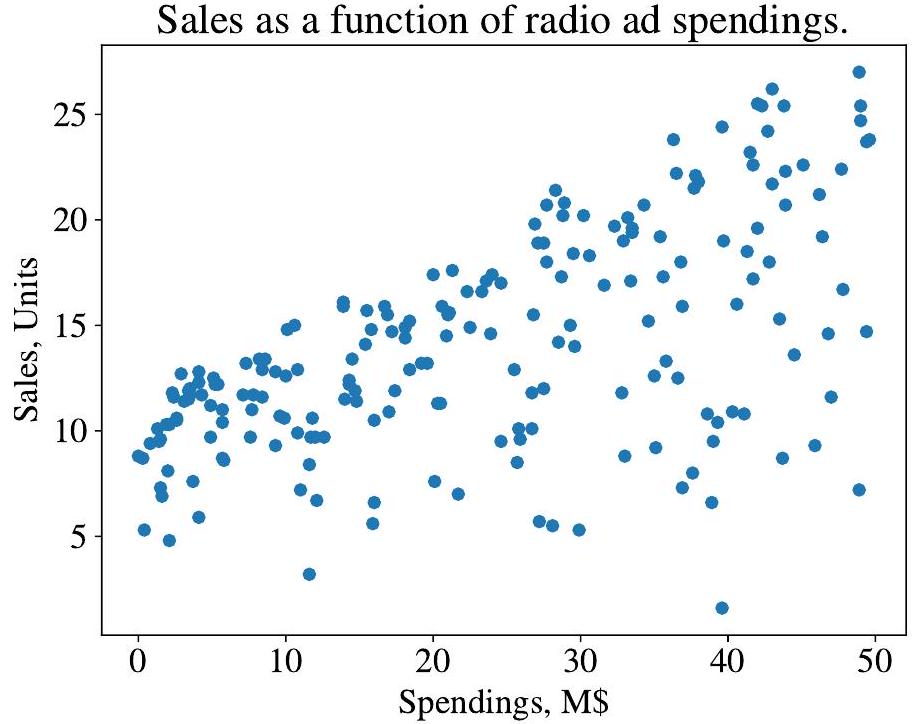
\includegraphics[width=0.5\textwidth]{imgs/ana_ml_1.jpeg}
		\caption{The original data. The Y-axis corresponds to the sales in units (the quantity we want to predict), the $\mathrm{X}$-axis corresponds to our feature: the spendings on radio ads in $\mathrm{M} \$$.}
	\end{figure}
\end{frame}

\begin{frame}
	Remember that the linear regression model looks like this: $f(x)=w x+b$. We don't know what the optimal values for $w$ and $b$ are and we want to learn them from data. To do that, we look for such values for $w$ and $b$ that minimize the mean squared error:
	$$
	l \stackrel{\text { def }}{=} \frac{1}{N} \sum_{i=1}^{N}\left(y_{i}-\left(w x_{i}+b\right)\right)^{2}
	$$
	Gradient descent starts with calculating the partial derivative for every parameter:
	
	$$
	\begin{aligned}
		\frac{\partial l}{\partial w} & =\frac{1}{N} \sum_{i=1}^{N}-2 x_{i}\left(y_{i}-\left(w x_{i}+b\right)\right) \\
		\frac{\partial l}{\partial b} & =\frac{1}{N} \sum_{i=1}^{N}-2\left(y_{i}-\left(w x_{i}+b\right)\right)
	\end{aligned}
	$$
\end{frame}

\begin{frame}
	$$
	\begin{aligned}
		\frac{\partial l}{\partial w} & =\frac{1}{N} \sum_{i=1}^{N}-2 x_{i}\left(y_{i}-\left(w x_{i}+b\right)\right) \\
		\frac{\partial l}{\partial b} & =\frac{1}{N} \sum_{i=1}^{N}-2\left(y_{i}-\left(w x_{i}+b\right)\right)
	\end{aligned}
	$$
	
	To find the partial derivative of the term $\left(y_{i}-(w x+b)\right)^{2}$ with respect to $w$ I applied the chain rule.
	\begin{itemize}
		\item Here, we have the chain $f=f_{2}\left(f_{1}\right)$ where $f_{1}=y_{i}-(w x+b)$ and $f_{2}=f_{1}^{2}$. 
		\item To find a partial derivative of $f$ with respect to $w$ we have to first find the partial derivative of $f$ with respect to $f_{2}$ which is equal to $2\left(y_{i}-(w x+b)\right)$ (from calculus, we know that the derivative $\left.\frac{\partial}{\partial x} x^{2}=2 x\right)$ and then we have to multiply it by the partial derivative of $y_{i}-(w x+b)$ with respect to $w$ which is equal to $-x$. So overall $\frac{\partial l}{\partial w}=\frac{1}{N} \sum_{i=1}^{N}-2 x_{i}\left(y_{i}-\left(w x_{i}+b\right)\right)$. 
	\end{itemize}
	 In a similar way, the partial derivative of $l$ with respect to $b, \frac{\partial l}{\partial b}$, was calculated.
\end{frame}

\begin{frame}
	Gradient descent proceeds in \textbf{epochs}. 
	\begin{itemize}
		\item An epoch consists of using the training set entirely to update each parameter. In the beginning, the first epoch, we initialize \footnote{In complex models, such as neural networks, which have thousands of parameters, the initialization of parameters may significantly affect the solution found using gradient descent. There are different initialization methods (at random, with all zeroes, with small values around zero, and others) and it is an important choice the data analyst has to make.} $ w \leftarrow 0$ and $b \leftarrow 0$. 
	\end{itemize}
	At each epoch, we update $w$ and $b$ using partial derivatives. The learning rate $\alpha$ controls the size of an update:
	
	$$
	\begin{gathered}
		w \leftarrow w-\alpha \frac{\partial l}{\partial w} \\
		b \leftarrow b-\alpha \frac{\partial l}{\partial b}
	\end{gathered}
	$$
	Because we want to minimize the objective function, when the derivative is positive we know that we need to move our parameter in the opposite direction (to the left on the axis of coordinates), vice versa. 
	
	At the next epoch, we recalculate partial derivatives with the updated values of $w$ and $b$; we continue the process until convergence. Typically, we need many epochs until we start seeing that the values for $w$ and $b$ don't change much after each epoch; then we stop.
\end{frame}

\begin{frame}
	\begin{columns}
		\column{0.5\textwidth}
			\begin{figure}
			\centering
			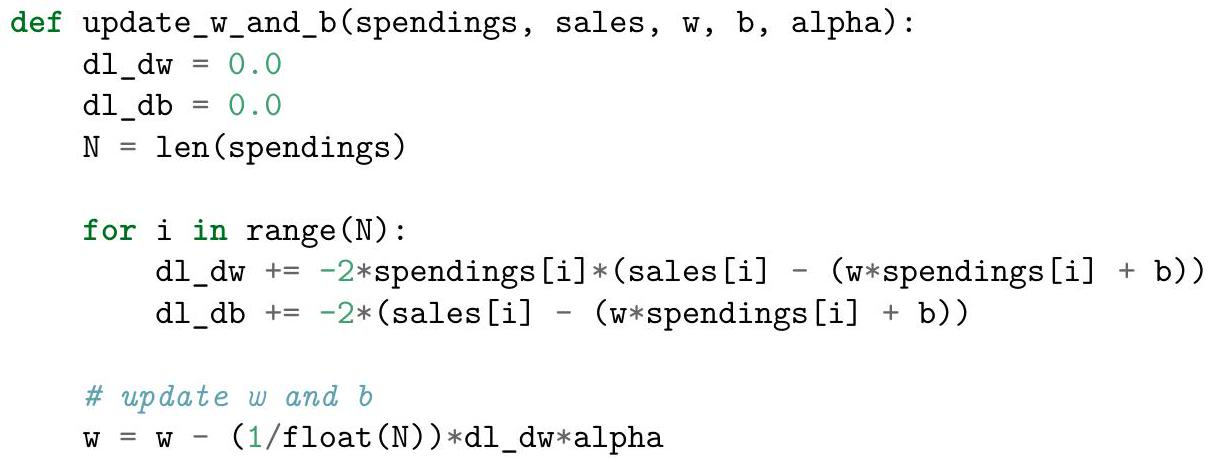
\includegraphics[width=\textwidth]{imgs/ana_ml_2.jpeg}
			\end{figure}
		\column{0.5\textwidth}
					\begin{figure}
					\centering
					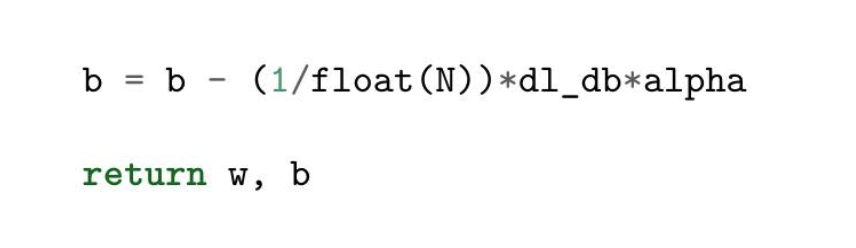
\includegraphics[scale=0.1]{imgs/ana_ml_3.png}
				\end{figure}
				The function that loops over multiple epochs is shown below:
				\begin{figure}
					\centering
					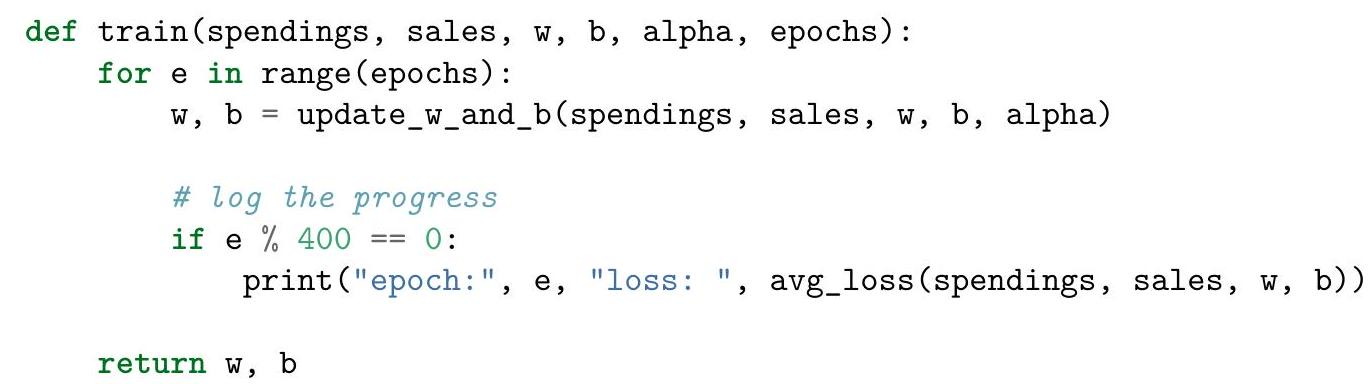
\includegraphics[width=\textwidth]{imgs/ana_ml_4.jpeg}
				\end{figure}
	\end{columns} 
\end{frame}

\begin{frame}
	\begin{figure}
		\centering
		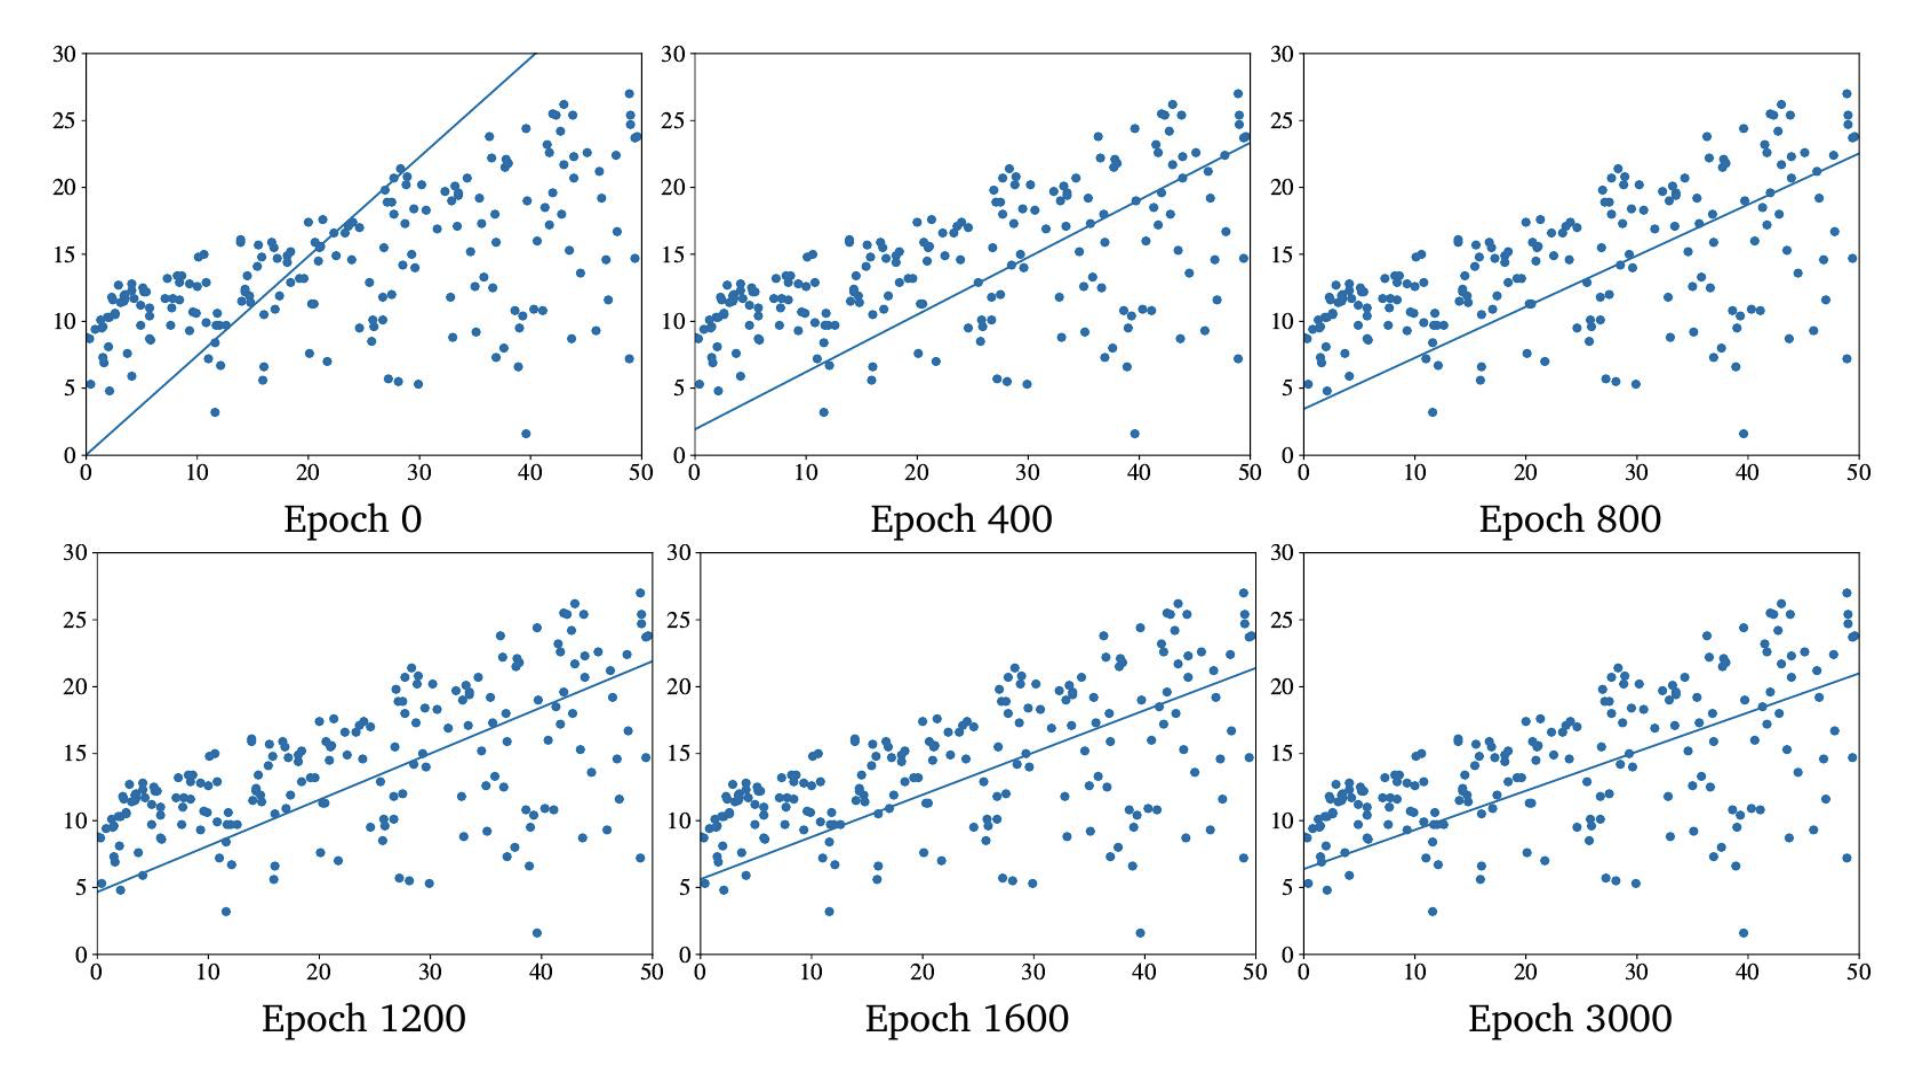
\includegraphics[width=\textwidth]{imgs/ana_ml_5.png}
		\caption{The evolution of the regression line through gradient descent epochs.}
	\end{figure}
\end{frame}

\begin{frame}
	If we run the \textit{train} function for $\alpha=0.001, w=0.0, b=0.0$, and 15,000 epochs, we will see the following output (shown partially):
	\begin{figure}
		\centering
		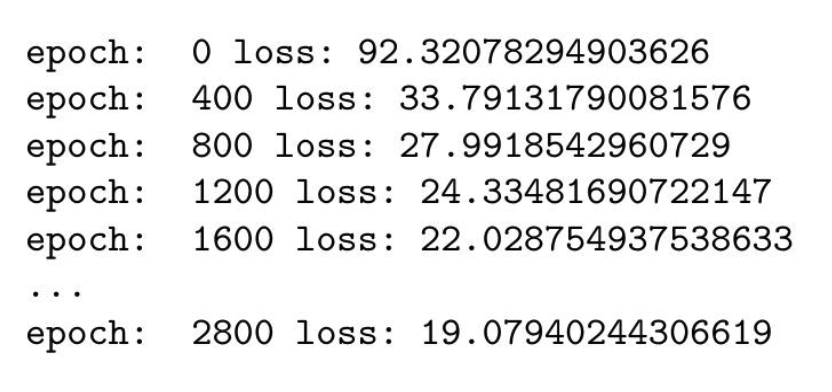
\includegraphics[width=0.5\textwidth]{imgs/ana_ml_6.png}
	\end{figure}
	You can see that the average loss decreases as the training function loops through epochs. 
\end{frame}

\begin{frame}
	Finally, once we have found the optimal values of parameters $w$ and $b$, the only missing piece is a function that makes predictions:
	\begin{figure}
		\centering
		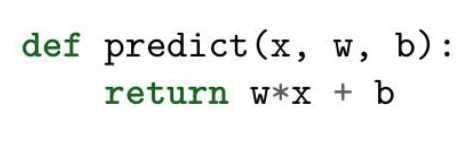
\includegraphics[width=0.3\textwidth]{imgs/ana_ml_7.png}
	\end{figure}
	Gradient descent is sensitive to the choice of the learning rate $\alpha$. It is also slow for large datasets. Fortunately, several significant improvements to this algorithm have been proposed.
	
	\textbf{Minibatch stochastic gradient descent} (minibatch SGD) is a version of the algorithm that speeds up the computation by approximating the gradient using smaller batches (subsets) of the training data. SGD itself has various "upgrades".
	\begin{itemize}
		\item  \textbf{Adagrad} is a version of SGD that scales $\alpha$ for each parameter according to the history of gradients. As a result, $\alpha$ is reduced for very large gradients and vice-versa.
		\item  \textbf{Momentum} is a method that helps accelerate SGD by orienting the gradient descent in the relevant direction and reducing oscillations.
	\end{itemize}
	 In neural network training, variants of SGD such as \textbf{RMSprop} and \textbf{Adam}, are very frequently used.
\end{frame}

\begin{frame}
	Notice that gradient descent and its variants are \textit{not} machine learning algorithms. They are solvers of minimization problems in which the function to minimize has a gradient (in most points of its domain).
\end{frame}

\section{Learning Algorithms' Particularities}
\begin{frame}{Learning Algorithms' Particularities}
	Here, I outline some practical particularities that can differentiate one learning algorithm from another. You already know that different learning algorithms can have different hyperparameters ( $C$ in SVM, $\epsilon$ and $d$ in ID3). Solvers such as gradient descent can also have hyperparameters, like $\alpha$ for example.
	
	\begin{itemize}
		\item Some algorithms, like decision tree learning, can accept categorical features. For example, if you have a feature "color" that can take values "red", "yellow", or "green", you can keep this feature as is. SVM, logistic and linear regression, as well as kNN (with cosine similarity or Euclidean distance metrics), expect numerical values for all features.
		\item Some algorithms, like SVM, allow the data analyst to provide weightings for each class. These weightings influence how the decision boundary is drawn. If the weight of some class is high, the learning algorithm tries to not make errors in predicting training examples of this class (typically, for the cost of making an error elsewhere). That could be important if instances of some class are in the minority in your training data, but you would like to avoid misclassifying examples of that class as much as possible.
	\end{itemize}
\end{frame}

\begin{frame}
	\begin{itemize}
		\item Some classification models, like SVM and kNN, given a feature vector only output the class. Others, like logistic regression or decision trees, can also return the score between 0 and 1 which can be interpreted as either how confident the model is about the prediction or as the probability that the input example belongs to a certain class.
		\item Some classification algorithms (like decision tree learning, logistic regression, or SVM) build the model using the whole dataset at once. If you have got additional labeled examples, you have to rebuild the model from scratch. Other algorithms (such as Naïve Bayes, multilayer perceptron, SGDClassifier/SGDRegressor, PassiveAggressiveClassifier/PassiveAggressiveRegressor in scikit-learn) can be trained iteratively, one batch at a time. Once new training examples are available, you can update the model using only the new data.
	\end{itemize}
\end{frame}

\begin{frame}
	\begin{itemize}
		\item Finally, some algorithms, like decision tree learning, SVM, and kNN can be used for both classification and regression, while others can only solve one type of problem: either classification or regression, but not both.
		\item Usually, each library provides the documentation that explains what kind of problem each algorithm solves, what input values are allowed and what kind of output the model produces. The documentation also provides information on hyperparameters.
	\end{itemize}
\end{frame}

\begin{frame}
    \begin{center}
        \Huge Questions?
    \end{center}
\end{frame}
\end{document}